\section{Isovector EMC Effects}

One aspect of the EMC effect that has not been fully explored are isovector-dependent effects.  Such effects would necessarily include degrees of freedom beyond the nuclear mass number $A$, which as has long been a method of parameterization~\cite{Malace:2014uea}.  In this situation, the nuclear $u_A$ and $d_A$ distributions can be modified separately, for example in an isovector mean field background or due to a preference in nucleon flavors in short range correlation pairing.  In a flavor separation which makes the assumption that $u_p = d_n$ and $d_p = u_n$ in the modified system, this manifests itself as an apparent charge symmetry breaking, though only by the assumption that protons and neutrons retain their local charge symmetry identity.  This is assumption is not necessarily true for a bound system and can be invalid for asymmetric nuclei in the same vein as the binding energy has a symmetry energy component.  Under the binding energy argument, as the symmetry energy is subleading to other bulk effects, such an isovector effect would be sub-leading to isoscalar modification effects.

The present world data have poor constraints on such an effect, in particular because many measurements of the EMC effect use symmetric or weakly asymmetric nuclei.  One calculation~\cite{Cloet:2009qs} using the Nambu-Jona-Lasinio (NJL) model and including the nuclear symmetry energy as an input, predicts deviations from the isoscalar EMC effect in the parton distribution functions on the order of several percent.   

Calculations based on short ranged correlations predict a similar picture~\cite{Sargsian:2012sm}.  The observed correspondence of the short range correlation plateau with the slope of the EMC effect would indicate local densities as a driving mechanism~\cite{PhysRevLett.106.052301}.  Using the observation that proton-neutron pairs are found much more frequently than neutron-neutron or proton-proton pairs~\cite{Subedi:2008zz} and simple counting arguments, modification of protons and neutrons will be different in nuclei depending on the asymmetry.  In either a mean field or short ranged correlation model, observation in the difference of quark flavors would require very high precision electromagnetic deep inelastic scattering measurements due to the suppression of the $d$ quark components by the square of the charges. 

Weak interactions offer a novel method to probe for these types of effects.  In charged-current processes, $u$ and $d$ quarks only participate in $W^-$ or $W^+$ exchange respectively and could be used to map out the flavor dependence.  The NuTeV experiment~\cite{Zeller:2001hh} was carried out using neutrino beams at Fermilab using the Paschos-Wolfenstein relation~\cite{Paschos:1972kj} to measure the weak mixing angle, $\sin^2\theta_\mathrm{W}$.  Due to the small neutrino cross section, heavy targets (iron) were employed which have a small neutron excess.  Charge symmetry in the bound nucleons was assumed and a significant deviation in $\sin^2\theta_\mathrm{W}$ was observed.  With the inclusion of an effect predicted by the NJL calculation noted above, much of the deviation is resolved.  Additionally, tension has been noted in nuclear PDF fits between neutrino data and other data sets which probe different flavor combinations~\cite{Schienbein:2009kk}.

\subsection{Flavor Dependence with Parity Violation}

The interference between electromagnetic and  neutral currents through parity-violating deep inelastic scattering can be used as a more precise measurement than available in electromagnetic scattering~\cite{Cloet:2012td}.  In this situation, a polarized lepton beam scattered from an unpolarized asymmetric nuclear target will form a small parity-violating cross section between the two beam helicity states, $\sigma_{\mathrm{L,R}}$, which is to leading order
\begin{equation}
        \frac{ \sigma_R - \sigma_L }{\sigma_R + \sigma_L} = -\frac{G_F Q^2}{4 \sqrt{2} \pi \alpha} \left[ Y_1 a_1(x) + Y_3(y) a_3(x) \right],
            \label{eq:phy:apv}
\end{equation}
where $G_F$ is the Fermi constant, $\alpha$ the fine structure constant, $x=Q^2/(2M\nu)$ the standard Bjorken-$x$ variable, $M$ the mass the of nucleon, $\nu$ the lepton energy transfer, and
\begin{equation}
        Y_1 \approx 1; \qquad Y_3(y) \approx \frac{1 - (1-y)^2}{1 + (1-y)^2}
    \end{equation}
    with
    \begin{eqnarray}
            a_1(x) & = &  2 \frac{ \sum_i C_{1i} e_i (q_i + \bar{q}_i) }{ \sum_i e_i^2 (q_i + \bar{q}_i) } \\
            a_3(x) & = &  2 \frac{ \sum_i C_{2i} e_i (q_i - \bar{q}_i) }{ \sum_i e_i^2 (q_i + \bar{q}_i) }. 
    \end{eqnarray}
    with $y=\nu/E$,  $E$ the beam energy, $e_i$ the quark electric charge couplings for flavor $i$, and $C_{1i}$ and $C_{2i}$ the effective quark couplings dependent on the weak-mixing angle $\sin^2\theta_\mathrm{W}$~\cite{Patrignani:2016xqp}.  The $a_1(x)$ term is dominant for fixed target, forward angle kinematics with $C_{1u} \approx -0.19$ and $C_{1d} \approx 0.34$.  An experimental proposal~\cite{emcpvdis} for the proposed SoLID spectrometer at Thomas Jefferson National Accelerator Facility would be able to test the difference between an NJL-sized effect and naive effect to better than 5-$\sigma$ using a ${}^{48}$Ca target, Fig.~\ref{fig:ivemc:pvdis}.

    \begin{figure}
        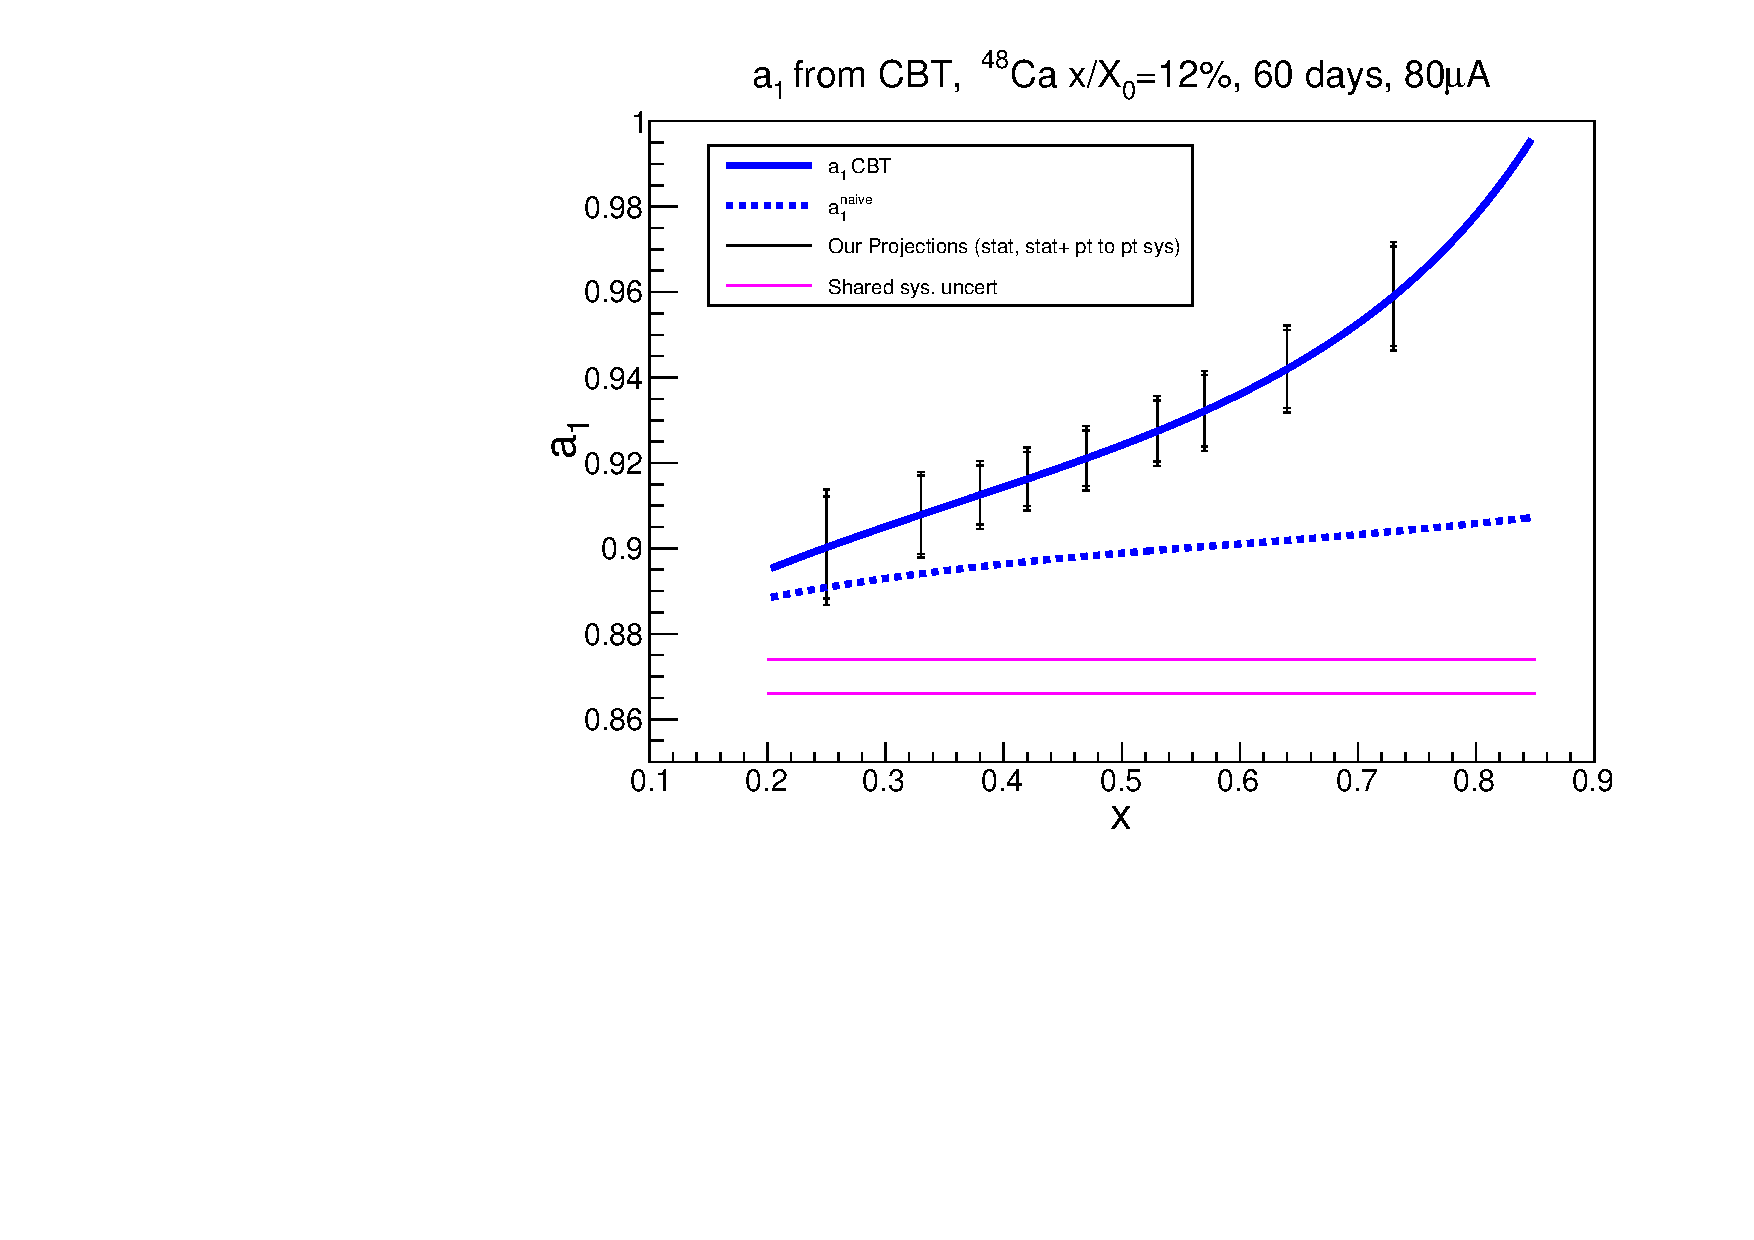
\includegraphics[width=0.5\textwidth]{plots/a1proj_2016.pdf}
        \caption{Projected sensitivities of the quantity $a_1$ for a proposed parity-violating deep inelastic scattering experiment~\cite{emcpvdis}.}
        \label{fig:ivemc:pvdis}
    \end{figure}





